\chapter{Dataset e Analisi esplorativa} \label{cap:dataset}
\section{Struttura del dataset}
Il dataset è composto da $13$ features estratte da un set di $3762$ immagini su
scala di grigi, ciascuna immagine è stata prodotta dalla risonanza magnetica del
cervello di diversi pazienti. Di conseguenza, si hanno un totale di $3762$
istanze, ognuna etichettata con un valore categorico che rappresenta la presenza
o meno del tumore al cervello. L'etichetta è presente nella colonna \textit{Class}
e assume i seguenti valori:
\begin{itemize}
      \item \textbf{Presenza del tumore}: $Class = 1$
      \item \textbf{Assenza del tumore}: $Class = 0$
\end{itemize}

Le features sono fornite insieme alle immagini e si presume che siano distribuite
secondo una distribuzione normale. Si presume inoltre che siano correttamente
associate alle immagini delle risonanze magnetiche corrispondenti \cite{explanation-features}.
Le caratteristiche si suddividono in:
\begin{enumerate}
      \item \textbf{First Order Features}: forniscono informazioni legate alle
            distribuzione dei livelli di grigio dell'immagine. Queste features
            corrispondono alle statistiche descrittive dei valori dei pixel
            che compongono l'immagine e corrispondono a:
            \begin{itemize}
                  \item \textbf{Media}.
                  \item \textbf{Varianza}.
                  \item \textbf{Deviazione standard}.
                  \item \textbf{Indice di asimmetria}.
                  \item \textbf{Indice di kurtosis}.
            \end{itemize}
      \item \textbf{Second Order Features}: forniscono informazioni sulla
            composizione della texture dell'immagine e si dividono in:
            \begin{itemize}
                  \item \textbf{Contrast}: misura la differenza tra i livelli di
                        grigio tra diverse parti dell'immagine. Maggiore sarà il
                        valore allora maggiore sarà la deviazione standard dei
                        livelli di grigio nell'immagine.
                  \item \textbf{Energy}: fornisce informazioni sulla texture e
                        sulla complessità. Maggiore sarà il valore di Energy,
                        allora maggiore sarà il contrasto oppure più dettagliata
                        sarà la texture.
                  \item \textbf{ASM}: misura quanto sono distribuiti uniformemente
                        i livelli di grigio nell'immagine. Maggiore sarà il valore
                        allora più uniforme sarà la distribuzione dei livelli di
                        grigio nell'immagine, quindi la variabilità dei livelli
                        di grigio è ridotta.
                  \item \textbf{Entropy}: misura la casualità dei livelli di
                        grigio, quindi l'entropia sarà massima quando tutti i
                        livelli di grigio sono equamente probabili (randomness).
                        Più precisamente immagini con un ampio range di valori
                        che i pixel assumono e un uniforme distribuzione di dei
                        valori dei pixel tendono ad aumentare il valore
                        dell'entropia.
                  \item \textbf{Homogeneous}: misura quanto sono uniformi i
                        livelli di grigio. Più alto sarà l'indice allora minore
                        sarà il contrasto dell'immagine.
                  \item \textbf{Dissimilarity}: misura quanto differiscono
                        diverse regioni dell'immagine. Un valore alto indica che
                        si hanno molte differenze tra diverse regioni della
                        stessa immagine, quindi più complessa sarà la texture.
                  \item \textbf{Correlation}: misura la correlazione dei livelli
                        di grigio tra diverse regioni della stessa immagine.
                  \item \textbf{Coarseness}: misura il grado di variazione o di
                        irregolarità dei livelli di grigio, quindi misura la
                        finezza o la granularità della texture.
            \end{itemize}
\end{enumerate}
\section{Analisi descrittiva}\label{sec:analisi-descrittiva}
Dopo aver esaminato la struttura del dataset e il significato delle
caratteristiche, è stato condotto un controllo per identificare la presenza di
valori nulli. Non sono stati rilevati valori nulli, pertanto non è stata
richiesta alcuna operazione per la gestione di tali valori. Successivamente, è
stato verificato se nel dataset fossero presenti valori duplicati, riscontrandone
un totale di $63$ che sono stati eliminati.

Dopo questa fase preliminare, è stata eseguita un'analisi della distribuzione
degli esempi in base alla classe di appartenenza al fine di valutare se il
dataset presentasse uno sbilanciamento. A tale scopo, è stato creato un
istogramma, illustrato nella figura \ref{fig:dist-classi}, che visualizza la
frequenza dei valori relativi all'attributo \textit{Class}.
\begin{figure}[!ht]
      \centering
      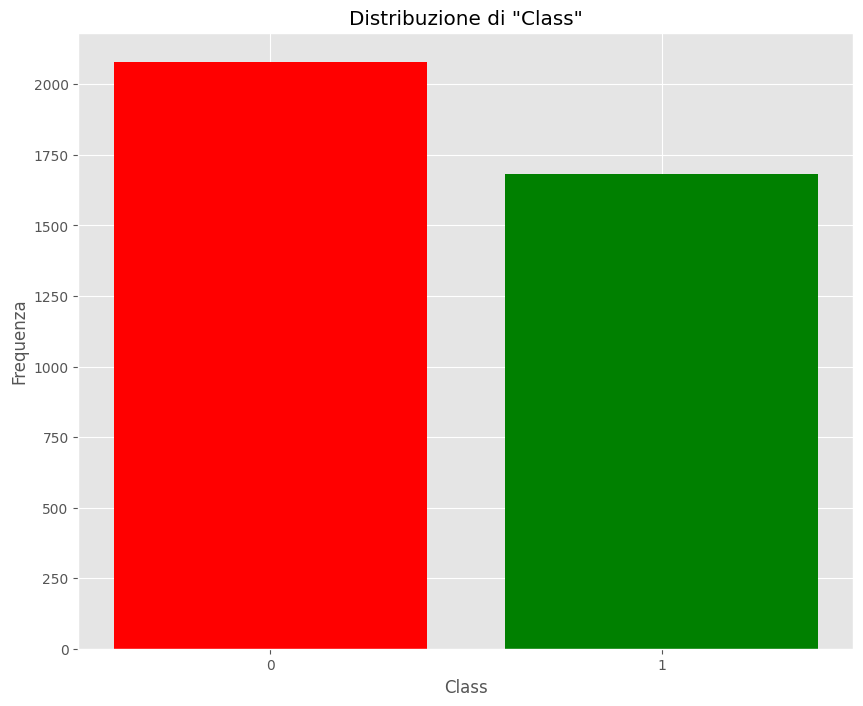
\includegraphics[width=0.5\textwidth]{img/analisi/distribuzioneClassi.png}
      \caption{Distribuzione delle classi}
      \label{fig:dist-classi}
\end{figure}

Dall'istogramma emerge un bilanciamento soddisfacente tra le classi, con il
$45\%$ degli esempi positivi, rappresentati in verde, e il $55\%$ degli esempi
negativi, evidenziati in rosso, nel dataset.

Dopo un'analisi della distribuzione relativa al valore del target, sono stati
generati $13$ istogrammi, presentati nella figura \ref{fig:barplot_features},
ciascuno dedicato a una specifica feature al fine di esaminarne la distribuzione
attraverso un'analisi visiva.
\begin{figure}[!ht]
      \centering
      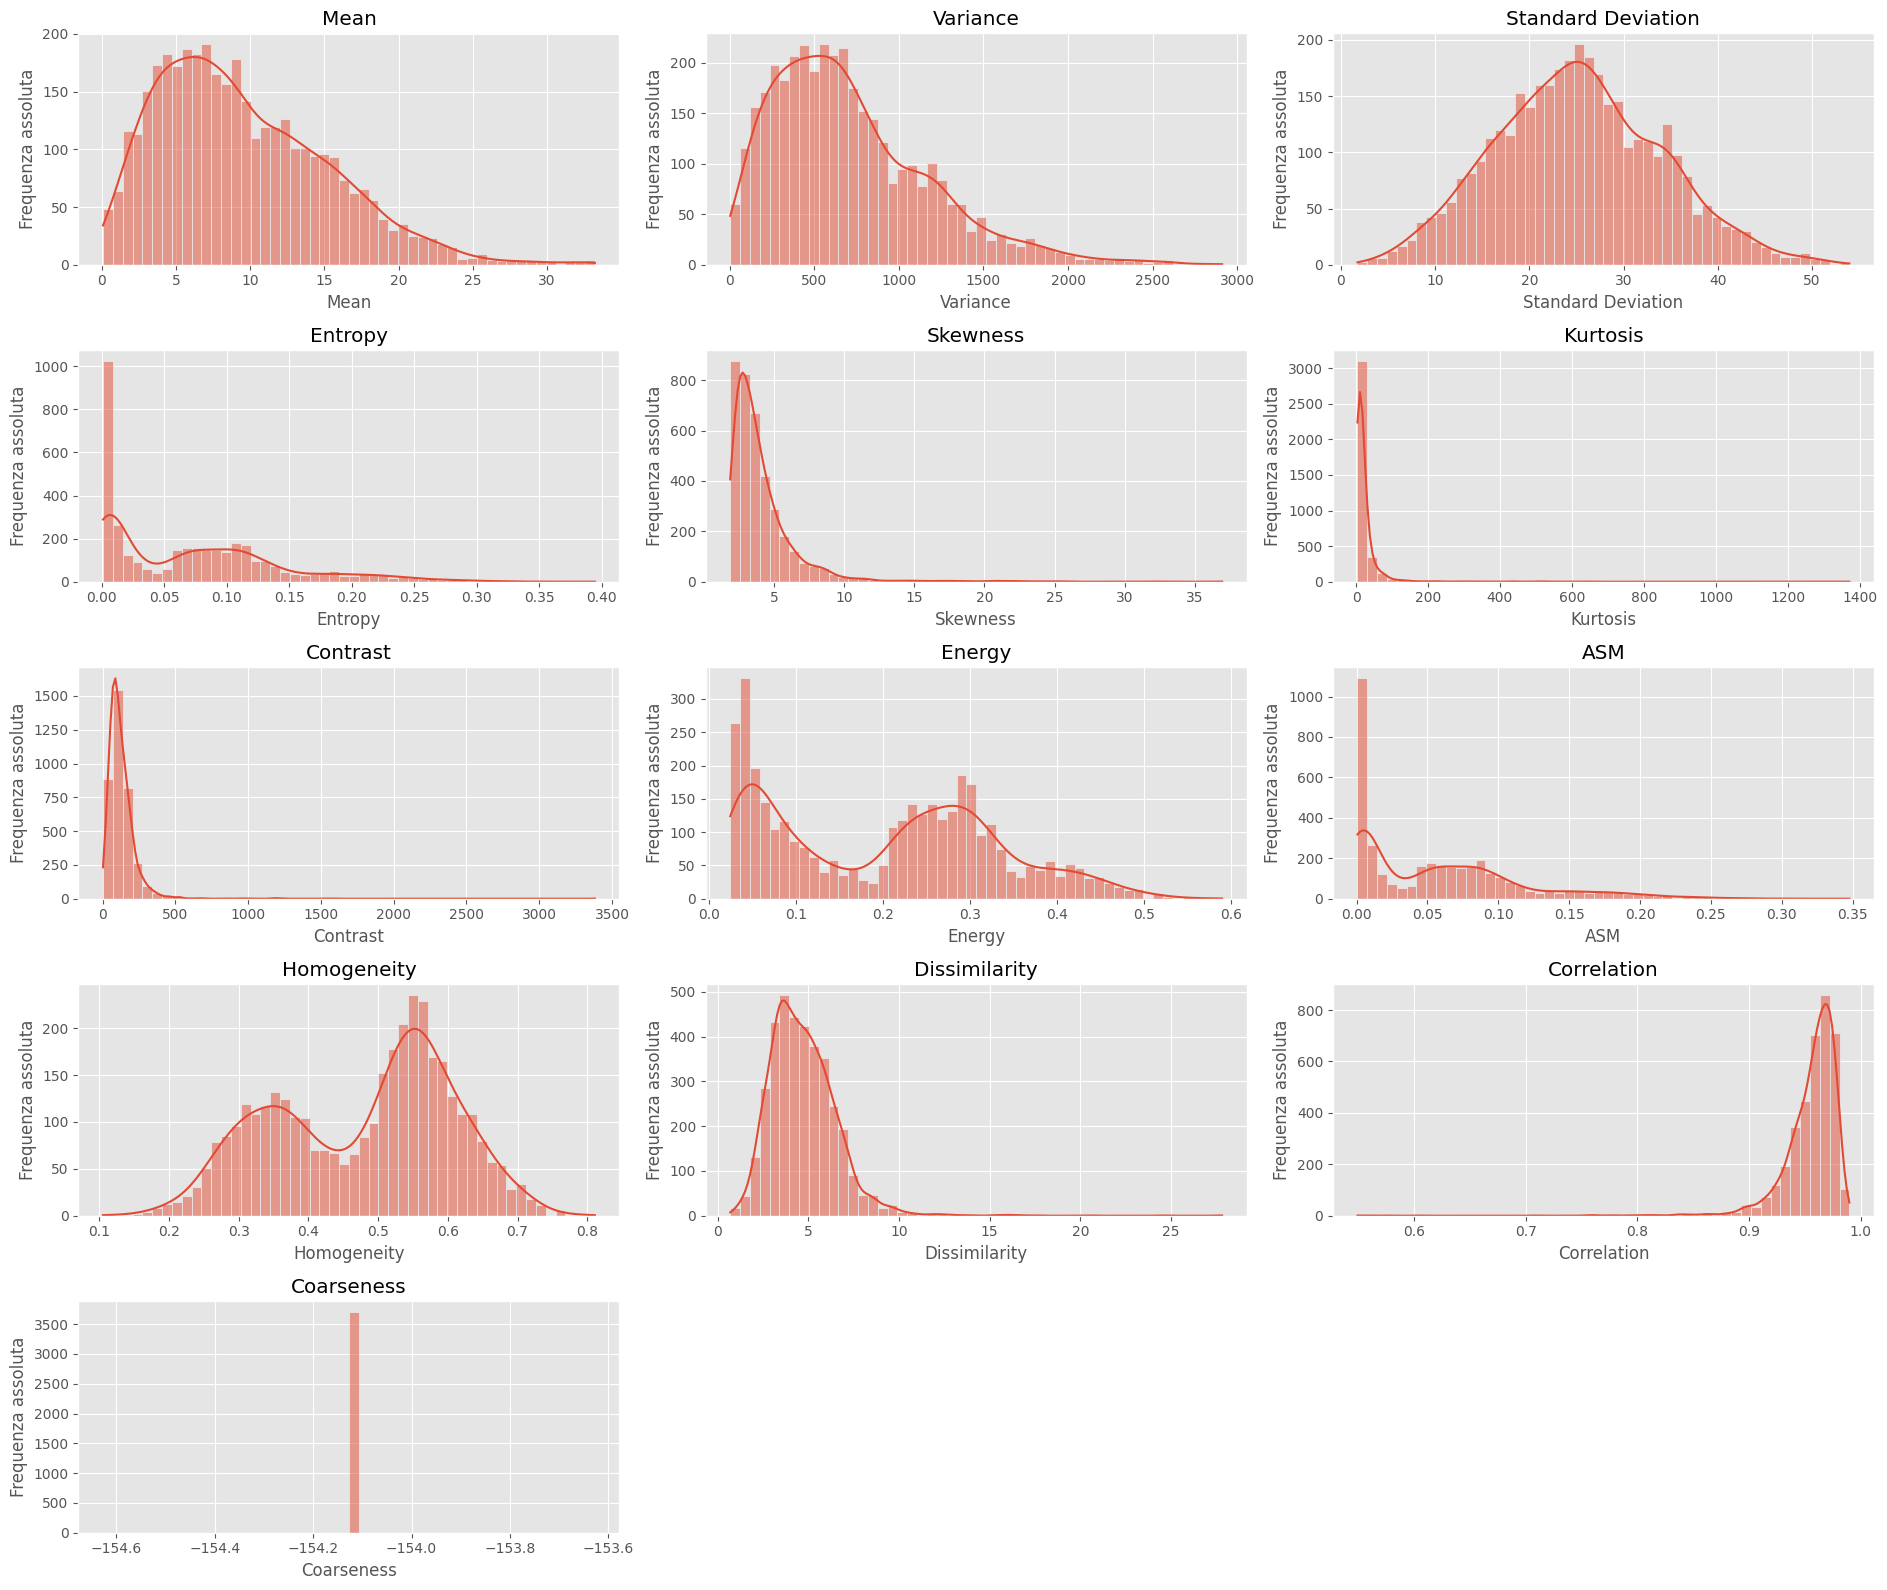
\includegraphics[width=\textwidth]{img/analisi/barplot.png}
      \caption{Istogramma delle features}
      \label{fig:barplot_features}
\end{figure}
L'analisi di tali grafici rivela che le features \textbf{Energy}, \textbf{ASM},
\textbf{Homogeneity}, \textbf{Entropy} e \textbf{Coarseness} non aderiscono a
una distribuzione normale, contrariamente alle altre feature le cui distribuzioni
mostrano un profilo più vicino alla distribuzione gaussiana. Tuttavia, nonostante
l'assenza di normalità in alcune features, si è deciso di non procedere con la
loro rimozione dal dataset. Invece, si è scelto di implementare i modelli senza
richiedere il rispetto delle loro ipotesi di normalità.

Inoltre, si nota che le features con una distribuzione simile a una normale non
sono state standardizzate, come indicato anche dalle statistiche descrittive
presentate nella tabella \ref{tab:desc-stat}
\begin{table}[!ht]
      \begin{subtable}[h]{1\textwidth}
            \centering
            \begin{tabular}{c|c c c c c c c c c c}
                  \hline
                  \rowcolor[HTML]{EFEFEF} \cellcolor[HTML]{EFEFEF}\textbf{} & \textbf{Mean} & \textbf{Variance} & \textbf{Standard Deviation} & \cellcolor[HTML]{EFEFEF}\textbf{Entropy} & \textbf{Skewness} & \textbf{Kurtosis} \\ \hline
                  \textbf{count}                                            & 3699          & 3699              & 3699                        & 3699                                     & 3699              & 3699              \\
                  \textbf{mean}                                             & 9.473354      & 710.895793        & 25.174138                   & 0.072940                                 & 4.108362          & 24.422551         \\
                  \textbf{std}                                              & 5.732700      & 468.154274        & 8.785183                    & 0.069914                                 & 2.559163          & 56.292660         \\
                  \textbf{min}                                              & 0.078659      & 3.145628          & 1.773592                    & 0.000882                                 & 1.886014          & 3.942402          \\
                  \textbf{25\%}                                             & 4.965988      & 362.568474        & 19.041231                   & 0.006662                                 & 2.621447          & 7.265711          \\
                  \textbf{50\%}                                             & 8.468414      & 624.708056        & 24.994160                   & 0.065681                                 & 3.422625          & 12.370334         \\
                  \textbf{75\%}                                             & 13.184586     & 967.036275        & 31.097207                   & 0.112694                                 & 4.662941          & 22.760735         \\
                  \textbf{max}                                              & 33.239975     & 2910.581879       & 53.949809                   & 0.394539                                 & 36.931294         & 1371.640060       \\ \hline
            \end{tabular}
            \caption{Statistiche descrittive delle feature \textit{Mean}, \textit{Variance}, \textit{Standard Deviation}, \textit{Entropy}, \textit{Skewness} e \textit{Kurtosis}.}
            \label{tab:primameta}
      \end{subtable}
      \hfill
      \begin{subtable}[h]{1\textwidth}
            \centering
            \resizebox{0.9\textwidth}{!}{\begin{tabular}{c|c c c c c c c c}
                        \hline
                        \rowcolor[HTML]{EFEFEF} \cellcolor[HTML]{EFEFEF}\textbf{} & \textbf{Contrast} & \textbf{Energy} & \textbf{ASM} & \textbf{Homogeneity} & \textbf{Dissimilarity} & \textbf{Correlation} & \textbf{Coarseness} \\ \hline
                        \textbf{count}                                            & 3699              & 3699            & 3699         & 3699                 & 3699                   & 3699                 & 3699                \\
                        \textbf{mean}                                             & 128.119746        & 0.203546        & 0.058080     & 0.478442             & 4.702774               & 0.955697             & 7.458341e-155       \\
                        \textbf{std}                                              & 110.168137        & 0.129047        & 0.057973     & 0.127971             & 1.856688               & 0.026061             & 0.000000e+00        \\
                        \textbf{min}                                              & 3.194733          & 0.024731        & 0.000612     & 0.105490             & 0.681121               & 0.549426             & 7.458341e-155       \\
                        \textbf{25\%}                                             & 72.057782         & 0.068793        & 0.004732     & 0.364279             & 3.413266               & 0.946879             & 7.458341e-155       \\
                        \textbf{50\%}                                             & 107.075103        & 0.223482        & 0.049944     & 0.511894             & 4.486111               & 0.961567             & 7.458341e-155       \\
                        \textbf{75\%}                                             & 161.199093        & 0.298110        & 0.088870     & 0.575239             & 5.725644               & 0.971315             & 7.458341e-155       \\
                        \textbf{max}                                              & 3382.574163       & 0.589682        & 0.347725     & 0.810921             & 27.827751              & 0.989972             & 7.458341e-155       \\ \hline
                  \end{tabular}}
            \caption{Statistiche descrittive delle feature \textit{Contrast}, \textit{Energy}, \textit{ASM}, \textit{Homogeneity}, \textit{Dissimilarity}, \textit{Correlation} e \textit{Coarseness}.}
            \label{tab:secondameta}
      \end{subtable}
      \caption{Statistiche descrittive degli attributi}
      \label{tab:desc-stat}
\end{table}
\newpage
Di conseguenza sarà opportuno standardizzare le features per rispettare le
assunzioni delle \textbf{SVM} e della \textbf{rete neurale}. Per quanto riguarda
\textbf{Gaussian Naive Bayes} non è necessario effettuare l'operazione
sopracitata, dal momento che nel calcolo della probabilità si sfrutta la formula
della Gaussiana nella quale viene fatta una standardizzazione implicita.

Dal calcolo delle statistiche descrittive si può osservare che la feature
\textbf{Coarseness} assume un valore poco significativo (tendente a $0$), quindi
si è pensato di convertire questa feature ad una scala logaritmica, permettendo
di aumentare la significatività dei valori. Nonostante questa trasformazione,
la feature presenta una deviazione standard nulla quindi questo suggerisce la
sua esclusione dal dataset in quanto sarà quasi sicuramente una feature poco
discriminante.

Durante la fase di analisi, risulta cruciale condurre uno studio sulla capacità
discriminante dei dati. A tale scopo, sono stati generati un totale di $13$
grafici, corrispondenti a ciascuna delle feature, ognuno dei quali è composto da 
due box plot che mostrano la suddivisione in percentili delle feature divise per 
le classi. Tali grafici sono visualizzabili nella figura \ref{fig:boxplot_features}.
\newpage
\begin{figure}[!ht]
      \centering
      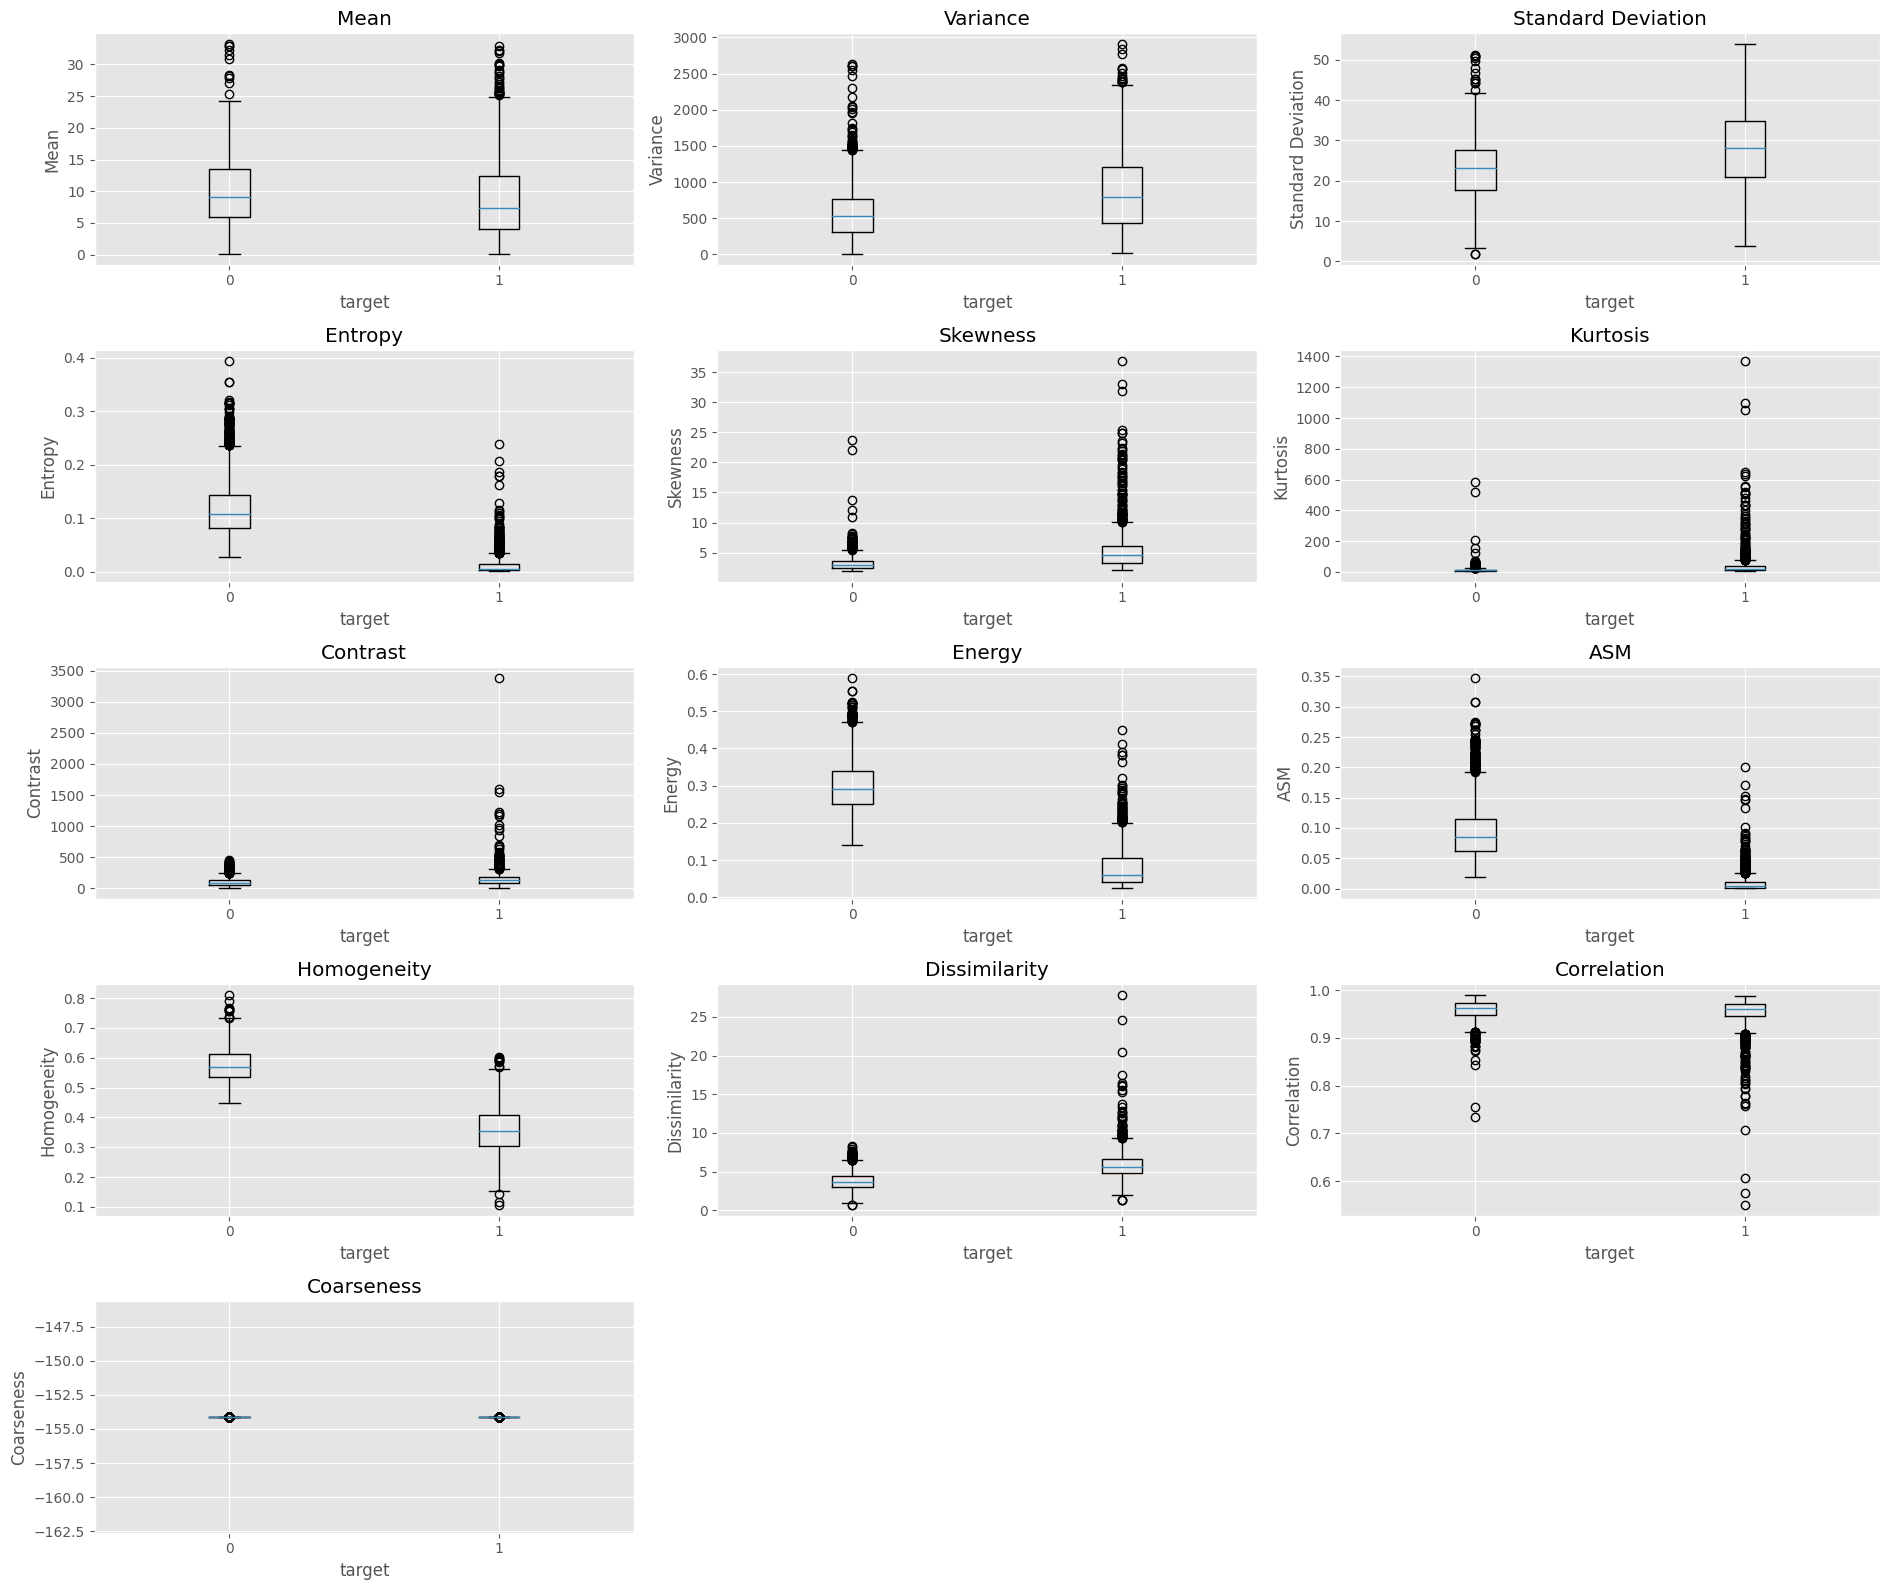
\includegraphics[width=\textwidth]{img/analisi/boxplot.png}
      \caption{Box plot delle features}
      \label{fig:boxplot_features}
\end{figure}

Dai box plot si può osservare che nel dataset sono presenti numerosi outliers, in
aggiunta le distribuzioni delle features separate per classi si sovrappongono
quasi tutte, eccetto per \textbf{Entropy}, \textbf{Energy}, \textbf{ASM} e
\textbf{Homogeneity}. Questo implica il fatto che potenzialmente sono le più
discriminanti rispetto alle altre features. I grafici confermano che l'attributo
\textbf{Coarseness} assume un valore costante, questo fornisce un'ulteriore
conferma per la sua rimozione dal dataset.

Al fine di concludere la fase di analisi, è stato condotto un confronto
sistematico delle features estratte a coppie al fine di valutare la possibilità
di separare linearmente le classi. A tal fine, sono state esaminate tutte le
possibili combinazioni di coppie di feature. Per ciascuna combinazione, è stato
generato un grafico cartesiano in cui ciascuna istanza è rappresentata da un
punto. Ogni punto sul grafico fornisce due informazioni fondamentali:
\begin{itemize}
      \item Il colore del punto specifica la classe di appartenenza dell'istanza.
      \item Le coordinate saranno i valori delle due features considerate.
\end{itemize}

I grafici evidenziano il fatto che per ogni coppia di features si ha almeno una
lieve sovrapposizione delle nuvole di punti rappresentanti le due classi, questo
significa che in due dimensioni le classi non sono linearmente separabili a meno
di accettare errori. In ogni caso, si possono osservare le coppie con
meno sovrapposizioni tra classi in questo caso sono:
\begin{itemize}
      \item \textit{Entropy} e \textit{Mean}
      \item \textit{Energy} e \textit{Mean}
      \item \textit{ASM} e \textit{Mean}
      \item \textit{Homogeneity} e \textit{Mean}
      \item \text{Entropy} e \textit{Variance}
      \item \textit{Energy} e \textit{Variance}
      \item \textit{ASM} e \textit{Variance}
      \item \textit{Standard Deviation} e \textit{Entropy}
      \item \textit{Standard Deviation} e \textit{Energy}
      \item \textit{Standard Deviation} e \textit{ASM}
\end{itemize}
Osservando queste coppie hanno un numero di istanze sovrapposte ridotto, allora
si può affermare che le SVM, con un kernel scelto in modo accurato, potrebbero
ottenere degli ottimi risultati nella classificazione. Inoltre, questi grafici
permettono anticipare dei primi studi sulla correlazione come la presenza di una
forte correlazione tra:
\begin{itemize}
      \item \textit{Mean} e \textit{Skewness}
      \item \textit{Variance} e \textit{Standard Deviation}: questa correlazione
            è facilmente spiegabile dal momento che la deviazione standard è la
            radice quadrata della varianza, quindi sono misure dipendenti.
      \item \textit{Entropy} e \textit{ASM}
      \item \textit{Entropy} e \textit{Energy}
      \item \textit{Skewness} e \textit{Kurtosis}
      \item \textit{Energy} e \textit{ASM}
\end{itemize}
\subsection{Analisi delle correlazioni} \label{sec:correlazione}
Il passaggio successivo è  stato quello di analizzare le correlazioni tra le
feature dal momento che un primo modo per ridurre la dimensionalità del dataset
è attraverso il mantenimento di solo una feature tra tutte quelle correlate.

Perciò per prima cosa è stata prodotta una matrice di correlazione, riportata in
figura \ref{fig:corr-matrix}, attraverso la quale è stato possibile osservare le
correlazioni tra le feature.
\begin{figure}[!ht]
      \centering
      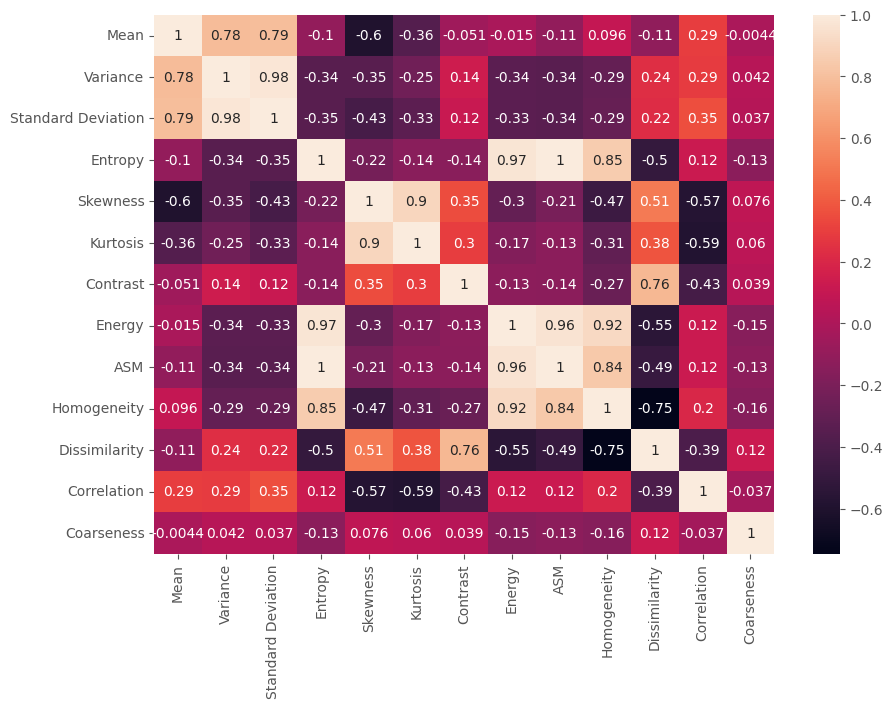
\includegraphics[width=0.5\textwidth]{img/analisi/corr.png}
      \caption{Matrice di correlazione}
      \label{fig:corr-matrix}
\end{figure}

Dall'analisi di questa matrice, si possono osservare diverse correlazioni tra le
feature. Innanzitutto, si può notare una forte correlazione positiva tra le
feature \textit{Mean}, \textit{Variance} e \textit{Standard deviation}. Questa
correlazione è facilmente spiegabile analizzando le immagini prodotte dalle
risonanze magnetiche. Infatti, essendo in bianco e nero, se la media tende a $1$
(colore bianco) allora la varianza e la deviazione standard aumentano, perché si
passa da pixel neri a pixel bianchi. Questo comporta che le transizioni dal nero
assoluto al bianco assoluto necessitano di regioni di pixel maggiore rispetto
ad una transizione tra nero assoluto e grigio ($0.5$).

Invece, la correlazione tra varianza è deviazione standard è facilmente spiegabile
perché la deviazione standard è la radice quadrata della varianza, quindi sono
misure dipendenti.

Una seconda forte correlazione positiva si può osservare tra le feature che
misurano l'\textbf{uniformità dei livelli di grigio} dei pixel, più precisamente
tra le feature \textit{Entropy}, \textit{ASM}, \textit{Homogeneity} ed
\textit{Energy}. Queste feature quantificano delle informazioni legate alla
texture dell'immagine, quindi la forte correlazione positiva può essere spiegata
analizzando le texture delle immagini su cui vengono calcolate. Più precisamente
se si ha un valore molto alto della feature \textit{Entropy}, significa che la
texture non è uniforme, ovvero si hanno strutture complesse e irregolari, quindi
più uniforme sarà la distribuzione dei livelli di grigio, aumentando l'indice
di \textit{ASM}, comportando di conseguenza un aumento delle variazioni di intensità
dei livelli di grigio, aumentando di conseguenza anche gli indici di \textit{Energy}
e \textit{Homogeneity}.

Al tempo stesso, la matrice di correlazione evidenza una forte correlazione positiva
tra gli indici che misurano la \textbf{morfologia della distribuzione dei livelli
      di grigio}, ovvero le feature di \textit{Skewness} e \textit{Kurtosis}.
Questa dipendenza implica il fatto che più la distribuzione è leptokurtica
(Kurtosis grande), ovvero la frequenza dei livelli di grigio dei pixel si
concentrano interamente vicino alla media/mediana/moda, allora più grande sarà
la Skewness, ovvero maggiore sarà la tendenza ad avere frequenze di livelli di
grigio più vicino al bianco (coda di destra più altra rispetto alla coda di
sinistra).

La matrice della correlazione evidenzia anche una correlazione positiva tra le
feature di \textit{Contrast} e \textit{Dissimilarity}, ovvero maggiore sarà il
contrasto e maggiore sarà la complessità della texture e quindi la metrica
\textit{Dissimilarity}.

In aggiunta dalla matrice si evidenza che le features di \textit{Dissimilarity}
e \textit{Homogeneity} sono correlate negativo, dal momento che una misura la
dissimilarità tra i livelli di grigio delle regioni e l'altra misura la loro
l'omogeneità.
\section{Riduzione di dimensionalità} \label{sec:riduzone_di_dimensionalità}
Dal momento che il dataset è composto da un totale di $13$ features, allora
è importante trovare il modo di ridurre la sua dimensionalità con lo scopo di
velocizzare l'apprendimento dei modelli e semplificare il task di classificazione.
Per ridurre la dimensionalità del dataset sono stati utilizzati due diversi metodi:
\begin{itemize}
      \item Riduzione basata sullo studio della correlazione delle features.
      \item Riduzione utilizzando la Principal Component Analysis (PCA).
\end{itemize}
\subsection{Riduzione con la correlazione} \label{sec:riduzione_correlazione}
Questo metodo si basa sulla correlazione delle features, ovvero se due features
sono correlate allora significa che a livello discriminante una delle due è
superflua, di conseguenza si può rimuovere.

Alla luce dello studio sulla correlazione effettuato nella sezione \ref{sec:correlazione},
è possibile ridurre la dimensionalità del dataset considerando solo una delle
features correlate, di conseguenza sono state considerate solo queste:
\begin{itemize}
      \item \textbf{Mean}
      \item \textbf{Entropy}
      \item \textbf{Skewness}
      \item \textbf{Contrast}
      \item \textbf{Correlation}
\end{itemize}
Il nuovo dataset così composto verrà chiamato \texttt{dataset\_corr} e dal momento
che \textbf{Entropy} è l'unico attributo che non segue una distribuzione standard,
allora si sottolinea che non verranno rispettate le assunzioni di normalità dei
$3$ modelli scelti. In aggiunta, dal momento che per le SVM e NN assumono di
lavorare su dati con distribuzione normale stanrdard, allora per essere più
compatibili possibili con le assunzioni, è stata creata una versione del dataset
normalizzata, chiamata \texttt{dataset\_corr\_std}.
\subsection{PCA} \label{sec:pca}
In seguito, è stato pensato di provare ad utilizzare un metodo di trasformazione
delle feature per ridurre la loro dimensionalità e successivamente analizzare i
risultati ottenuti. La scelta sul metodo da utilizzare è ricaduta su \textbf{PCA}.

Prima di applicare la PCA, è stato necessario standardizzare le feature del dataset
originario senza i duplicati, ma con l'attributo \textbf{Coarseness}, dal momento
che se ne occuperà PCA della sua rimozione. In aggiunta, l'operazione di
standardizzazione è necessaria per evitare che le feature con varianza maggiore
abbiano un peso maggiore rispetto alle altre. Senza standardizzare delle feature,
la PCA potrebbe non essere in grado di trovare le direzioni di massima varianza.

La prima parte dell'analisi è stata quella di trovare il corretto numero di
componenti da utilizzare per la PCA. Questo è stato fatto attraverso
l'osservazione della percentuale di varianza spiegata per ogni componente. Per
svolgere questa operazione sono state utilizzate solamente le feature numeriche
del dataset, quindi sono state escluse le colonne \textit{Image} e \textit{Class}.

Rimosse le colonne non necessarie, è stato possibile computare la PCA utilizzando
la libreria \textit{sklearn} e successivamente è stato possibile osservare la
percentuale di varianza spiegata per ogni componente, riportata in figura \ref{fig:pca}.
\begin{figure}[!ht]
      \centering
      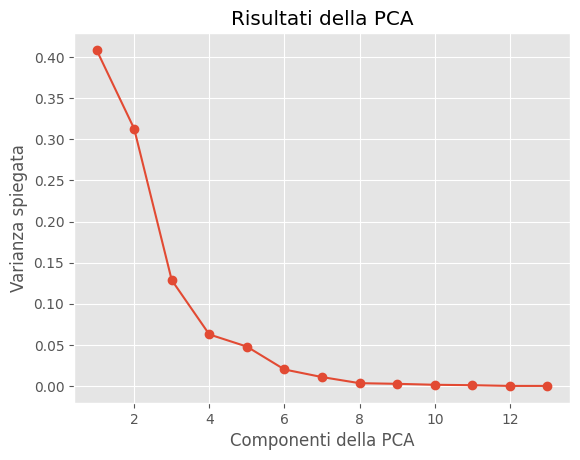
\includegraphics[width=0.45\textwidth]{img/analisi/pcaVarianza.png}
      \caption{Percentuale di varianza spiegata per ogni componente}
      \label{fig:pca}
\end{figure}

Dall'analisi della percentuale di varianza spiegata per ogni componente, si può
osservare che le prime $3$ componenti spiegano circa l'$85\%$ della varianza
dei dati. Questo ci ha permesso di ridurre la dimensionalità del dataset a soli
$3$ attributi, permettendo di rappresentare i dati in uno spazio a $3$ dimensioni.
\begin{figure}[!ht]
      \centering
      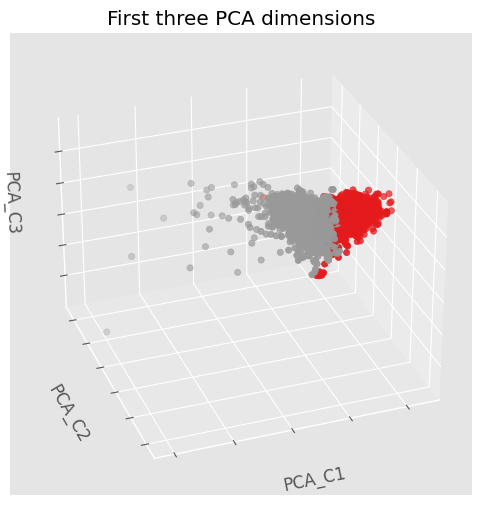
\includegraphics[width=0.4\textwidth]{img/analisi/pcaNuovoDataset.png}
      \caption{Scatter plot a 3 dimensioni}
      \label{fig:pca-3d}
\end{figure}

Dalla figura \ref{fig:pca-3d} si può osservare che i dati ottenuti dalla PCA
sembrano essere separabili con un iperpiano. Il nuovo dataset ridotto verrà
denominato \texttt{dataset\_pca} e dal momento che SVM e NN hanno bisogno di dati
standardizzati, allora è stato prodotto anche la sua versione standardizzata,
chiamata \texttt{dataset\_pca\_std}.

% \section{Preparazione dei dati} \label{sec:preparazione_dei_dati}
% Terminata la fase di riduzione della dimensionalità, si è passati alla fase di 
% preparazione dei dati per l'addestramento dei modelli. Dal momento che sono state 
% create nuove versioni del dataset di partenza, allora è stata prodotta la tabella 
% \ref{tab:riassunto_operazioni_dataset} come riepilogo dei dataset prodotti.

% dataset differenti, due valutazioni diverse, la prima su una suddivisione $80-20$, 
% la seconda una cross-validation sull'intero dataset. Allora è sta

% La strategia di valutazione dei modelli si è basata sull'esecuzione sequenziale 
% dei seguenti passi:
% \begin{itemize}
%       \item \textbf{valutazione classica}: apprendimento del modello su $80\%$ del
%       dataset e valutazione sul $20\%$ del dataset rimanente
%       \item \textbf{cross-validation}: validazione del modello utilizzando 
%       $10$ fold stratified cross-validation
% \end{itemize}

% Perciò a causa della prima valutazione è stata applicata una suddivisione 
% stratificata $80-20$ di tutti i dataset ridotti, ovvero su 
% \texttt{dataset\_corr}, \texttt{dataset\_corr\_std}, \texttt{dataset\_pca}
% e \texttt{dataset\_pca\_std}. La suddivisione è stata effettuata in modo stratificato
% per mantenere bilanciate le classi sia nell'insieme di train, sia nell'insieme di test.
% Inoltre, per l'apprendimento dei modelli è stato necessario effettuare una ricerca
% degli iperparametri migliori, quindi è stata effettuata una \textit{cross-validation} 
% sul training set ottenuto precedentemente, più precisamente si è scelto di utilizzare 
% una k-fold cross-validation con k=5.

% La standardizzazione dei dati è stata effettuata in quanto la rete neurale e
% la SVM sono modelli che possono essere influenzati dalla distribuzione dei dati.
